\documentclass[11pt, a4paper]{article}
\usepackage{pdfpages}
\usepackage{parallel}
\usepackage[T2A]{fontenc}
\usepackage{ucs}
\usepackage[utf8x]{inputenc}
\usepackage[polish,english,russian]{babel}
\usepackage{hyperref}
\usepackage{rotating}
\usepackage[inner=2cm,top=1.8cm,outer=2cm,bottom=2.3cm,nohead]{geometry}
\usepackage{listings}
\usepackage{graphicx}
\usepackage{wrapfig}
\usepackage{longtable}
\usepackage{indentfirst}
\usepackage{array}
\usepackage{tikzsymbols}
\usepackage{soul}
\usepackage[ruled,vlined]{algorithm2e}
%\counterwithout{figure}{section} 

\usepackage{url}
\makeatletter
\g@addto@macro{\UrlBreaks}{\UrlOrds}
\makeatother

\newcolumntype{P}[1]{>{\raggedright\arraybackslash}p{#1}}
\frenchspacing
\usepackage{fixltx2e} %text sub- and superscripts
\usepackage{icomma} % коскі ў матэматычным рэжыме
\PreloadUnicodePage{4}

\newcommand{\longpage}{\enlargethispage{\baselineskip}}
\newcommand{\shortpage}{\enlargethispage{-\baselineskip}}

\def\switchlang#1{\expandafter\csname switchlang#1\endcsname}
\def\switchlangbe{
\let\saverefname=\refname%
\def\refname{Літаратура}%
\def\figurename{Іл.}%
}
\def\switchlangen{
\let\saverefname=\refname%
\def\refname{References}%
\def\figurename{Fig.}%
}
\def\switchlangru{
\let\saverefname=\refname%
\let\savefigurename=\figurename%
\def\refname{Литература}%
\def\figurename{Рис.}%
}

\hyphenation{admi-ni-stra-tive}
\hyphenation{ex-pe-ri-ence}
\hyphenation{fle-xi-bi-li-ty}
\hyphenation{Py-thon}
\hyphenation{ma-the-ma-ti-cal}
\hyphenation{re-ported}
\hyphenation{imp-le-menta-tions}
\hyphenation{pro-vides}
\hyphenation{en-gi-neering}
\hyphenation{com-pa-ti-bi-li-ty}
\hyphenation{im-pos-sible}
\hyphenation{desk-top}
\hyphenation{elec-tro-nic}
\hyphenation{com-pa-ny}
\hyphenation{de-ve-lop-ment}
\hyphenation{de-ve-loping}
\hyphenation{de-ve-lop}
\hyphenation{da-ta-ba-se}
\hyphenation{plat-forms}
\hyphenation{or-ga-ni-za-tion}
\hyphenation{pro-gramming}
\hyphenation{in-stru-ments}
\hyphenation{Li-nux}
\hyphenation{sour-ce}
\hyphenation{en-vi-ron-ment}
\hyphenation{Te-le-pathy}
\hyphenation{Li-nux-ov-ka}
\hyphenation{Open-BSD}
\hyphenation{Free-BSD}
\hyphenation{men-ti-on-ed}
\hyphenation{app-li-ca-tion}

\def\progref!#1!{\texttt{#1}}
\renewcommand{\arraystretch}{2} %Іначай формулы ў матрыцы зліпаюцца з лініямі
\usepackage{array}

\def\interview #1 (#2), #3, #4, #5\par{

\section[#1, #3, #4]{#1 -- #3, #4}
\def\qname{LVEE}
\def\aname{#1}
\def\q ##1\par{{\noindent \bf \qname: ##1 }\par}
\def\a{{\noindent \bf \aname: } \def\qname{L}\def\aname{#2}}
}

\def\interview* #1 (#2), #3, #4, #5\par{

\section*{#1\\{\small\rm #3, #4. #5}}
\ifx\ParallelWhichBox\undefined%
    \addcontentsline{toc}{section}{#1, #3, #4}%
\else%
\ifnum\ParallelWhichBox=0%
    \addcontentsline{toc}{section}{#1, #3, #4}%
\fi\fi%

\def\qname{LVEE}
\def\aname{#1}
\def\q ##1\par{{\noindent \bf \qname: ##1 }\par}
\def\a{{\noindent \bf \aname: } \def\qname{L}\def\aname{#2}}
}

\newcommand{\interviewfooter}[1]{
\vskip 1em
\noindent \textit{#1}
}

\switchlang{en}
\begin{document}

\title{1986 "--- Commodore C300 mouse}
\date{}
\maketitle
\selectlanguage{english}
The Commodore C300 mouse labeled Joystick Mouse on the box is one of the reincarnations of the Kempston Mouse released in 1986 for ZX Spectrum computers \cite{SinclairUser}, adapted for Commodore computers \cite{c64wiki}. Externally, the mouse looks typical, having two buttons on top and a ball on the bottom (figure \ref{fig:C300Pic}).

\begin{figure}[h]
    \centering
    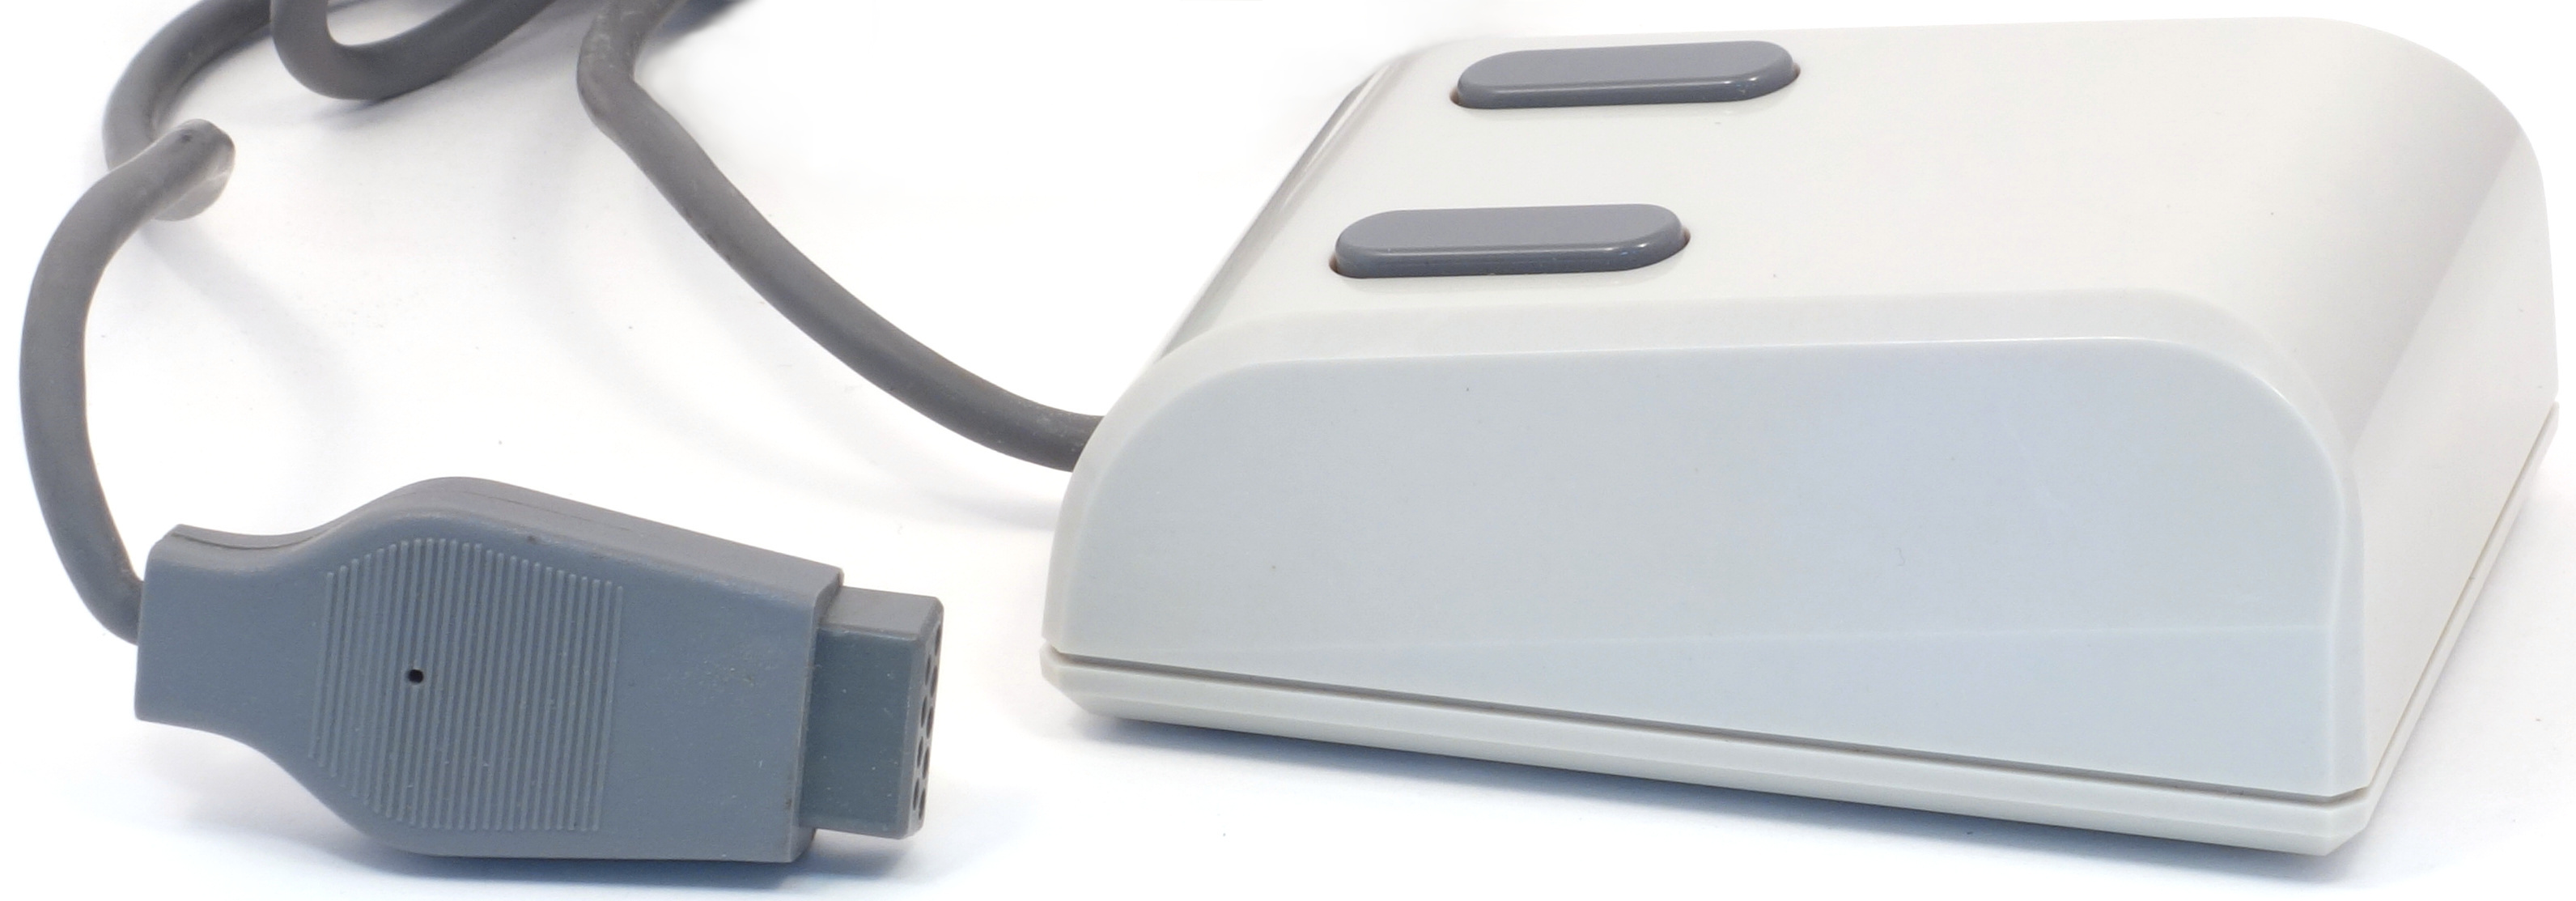
\includegraphics[scale=0.7]{1986_commodore_c300_mouse/cmnirm_30.jpg}
    \caption{Commodore C300 Mouse}
    \label{fig:C300Pic}
\end{figure}

According to the accompanying description, this mouse has two modes of operation: joystick mode and proportional mode. The operating mode is determined when the computer is turned on: the pressed right mouse button turns on the joystick mode, otherwise (by default) the mouse works in proportional mode. In joystick mode, the left mouse button is used as the joystick button, and the right button is equivalent to moving the joystick up. Joystick mode allows you to use the mouse with any joystick-compatible software, and also acts as a "fallback" in case the software you are using does not support proportional mode.

\begin{figure}[h]
    \centering
    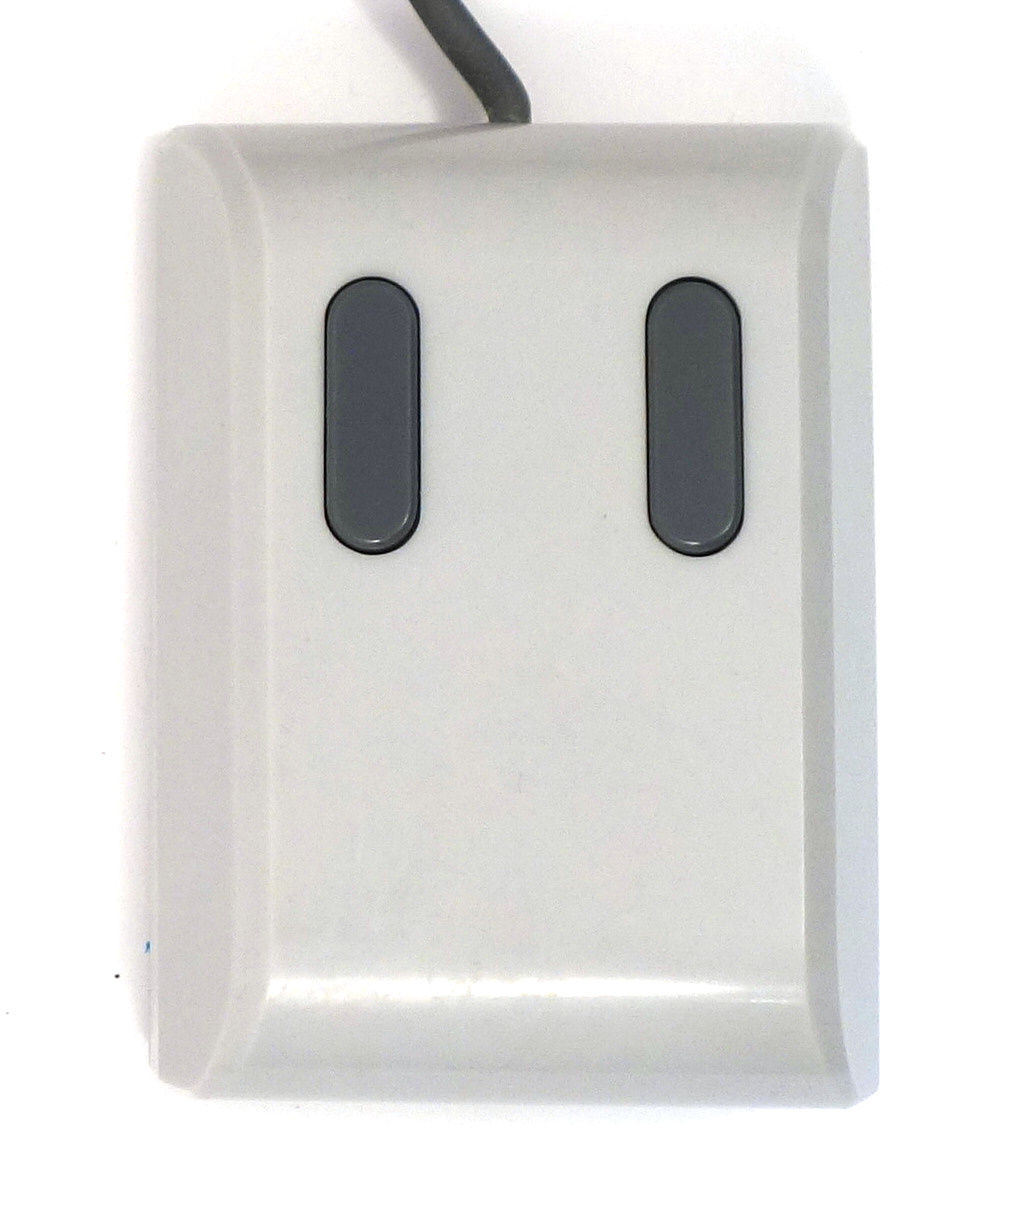
\includegraphics[scale=0.75]{1986_commodore_c300_mouse/3verh_60.jpg}
    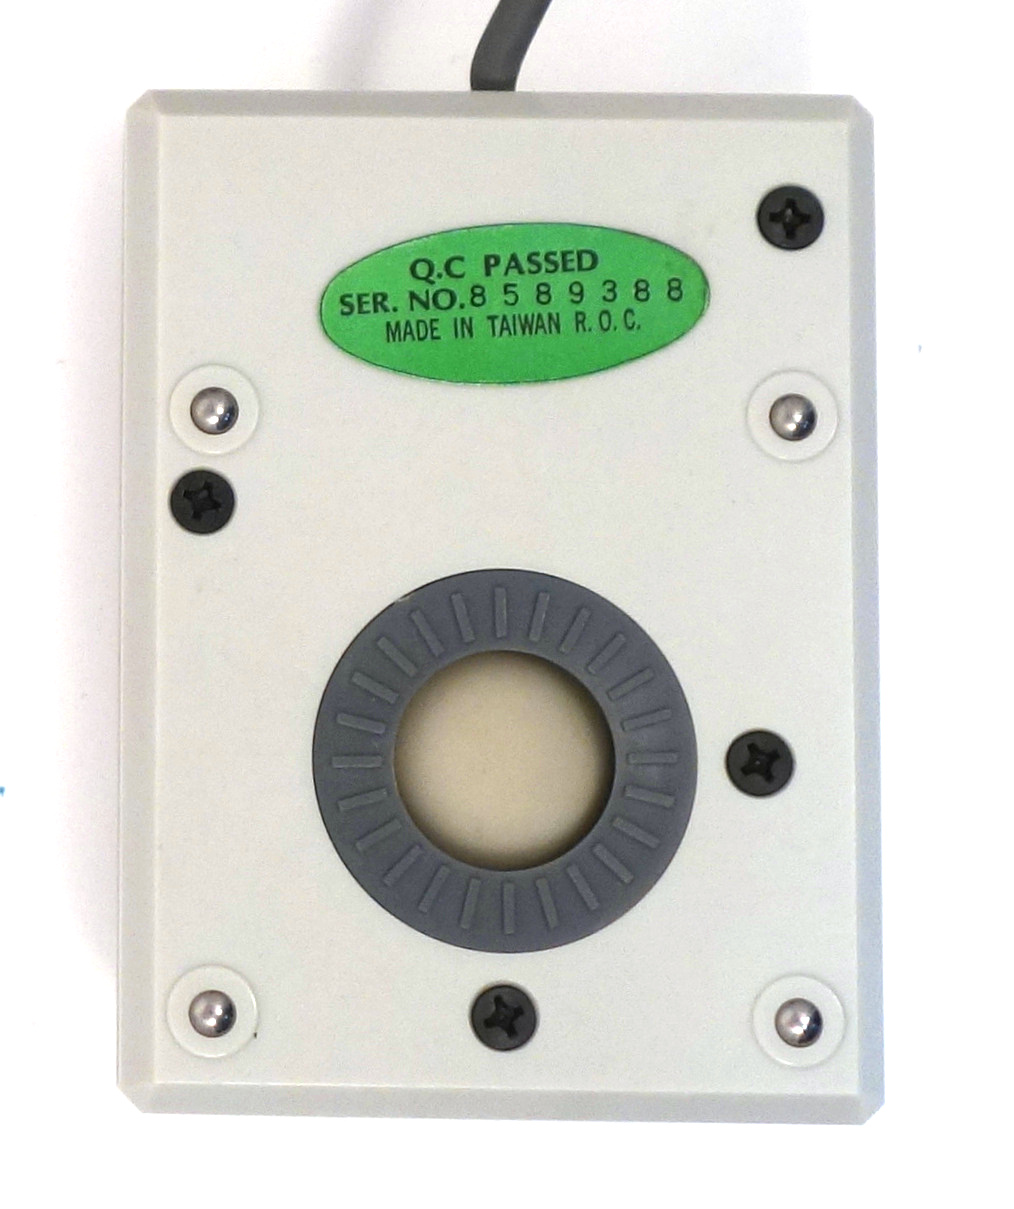
\includegraphics[scale=0.75]{1986_commodore_c300_mouse/3niz_60.jpg}
    \caption{Commodore C300 Mouse, top and bottom views}
    \label{fig:C300TopAndBottom}
\end{figure}

As you can see in figure \ref{fig:C300TopAndBottom}, the smooth glide of the mouse over the work surface is provided not by low-resistance fabric pads or plastic <<feet>>, but by four small-diameter metal balls located in additional holes on the bottom side of the case, which rotate freely when moving (a solution typical for a number of mechanical mice of the 80s, produced before the change in the standard design, aimed at reducing the cost of products).

\begin{figure}[h]
    \centering
    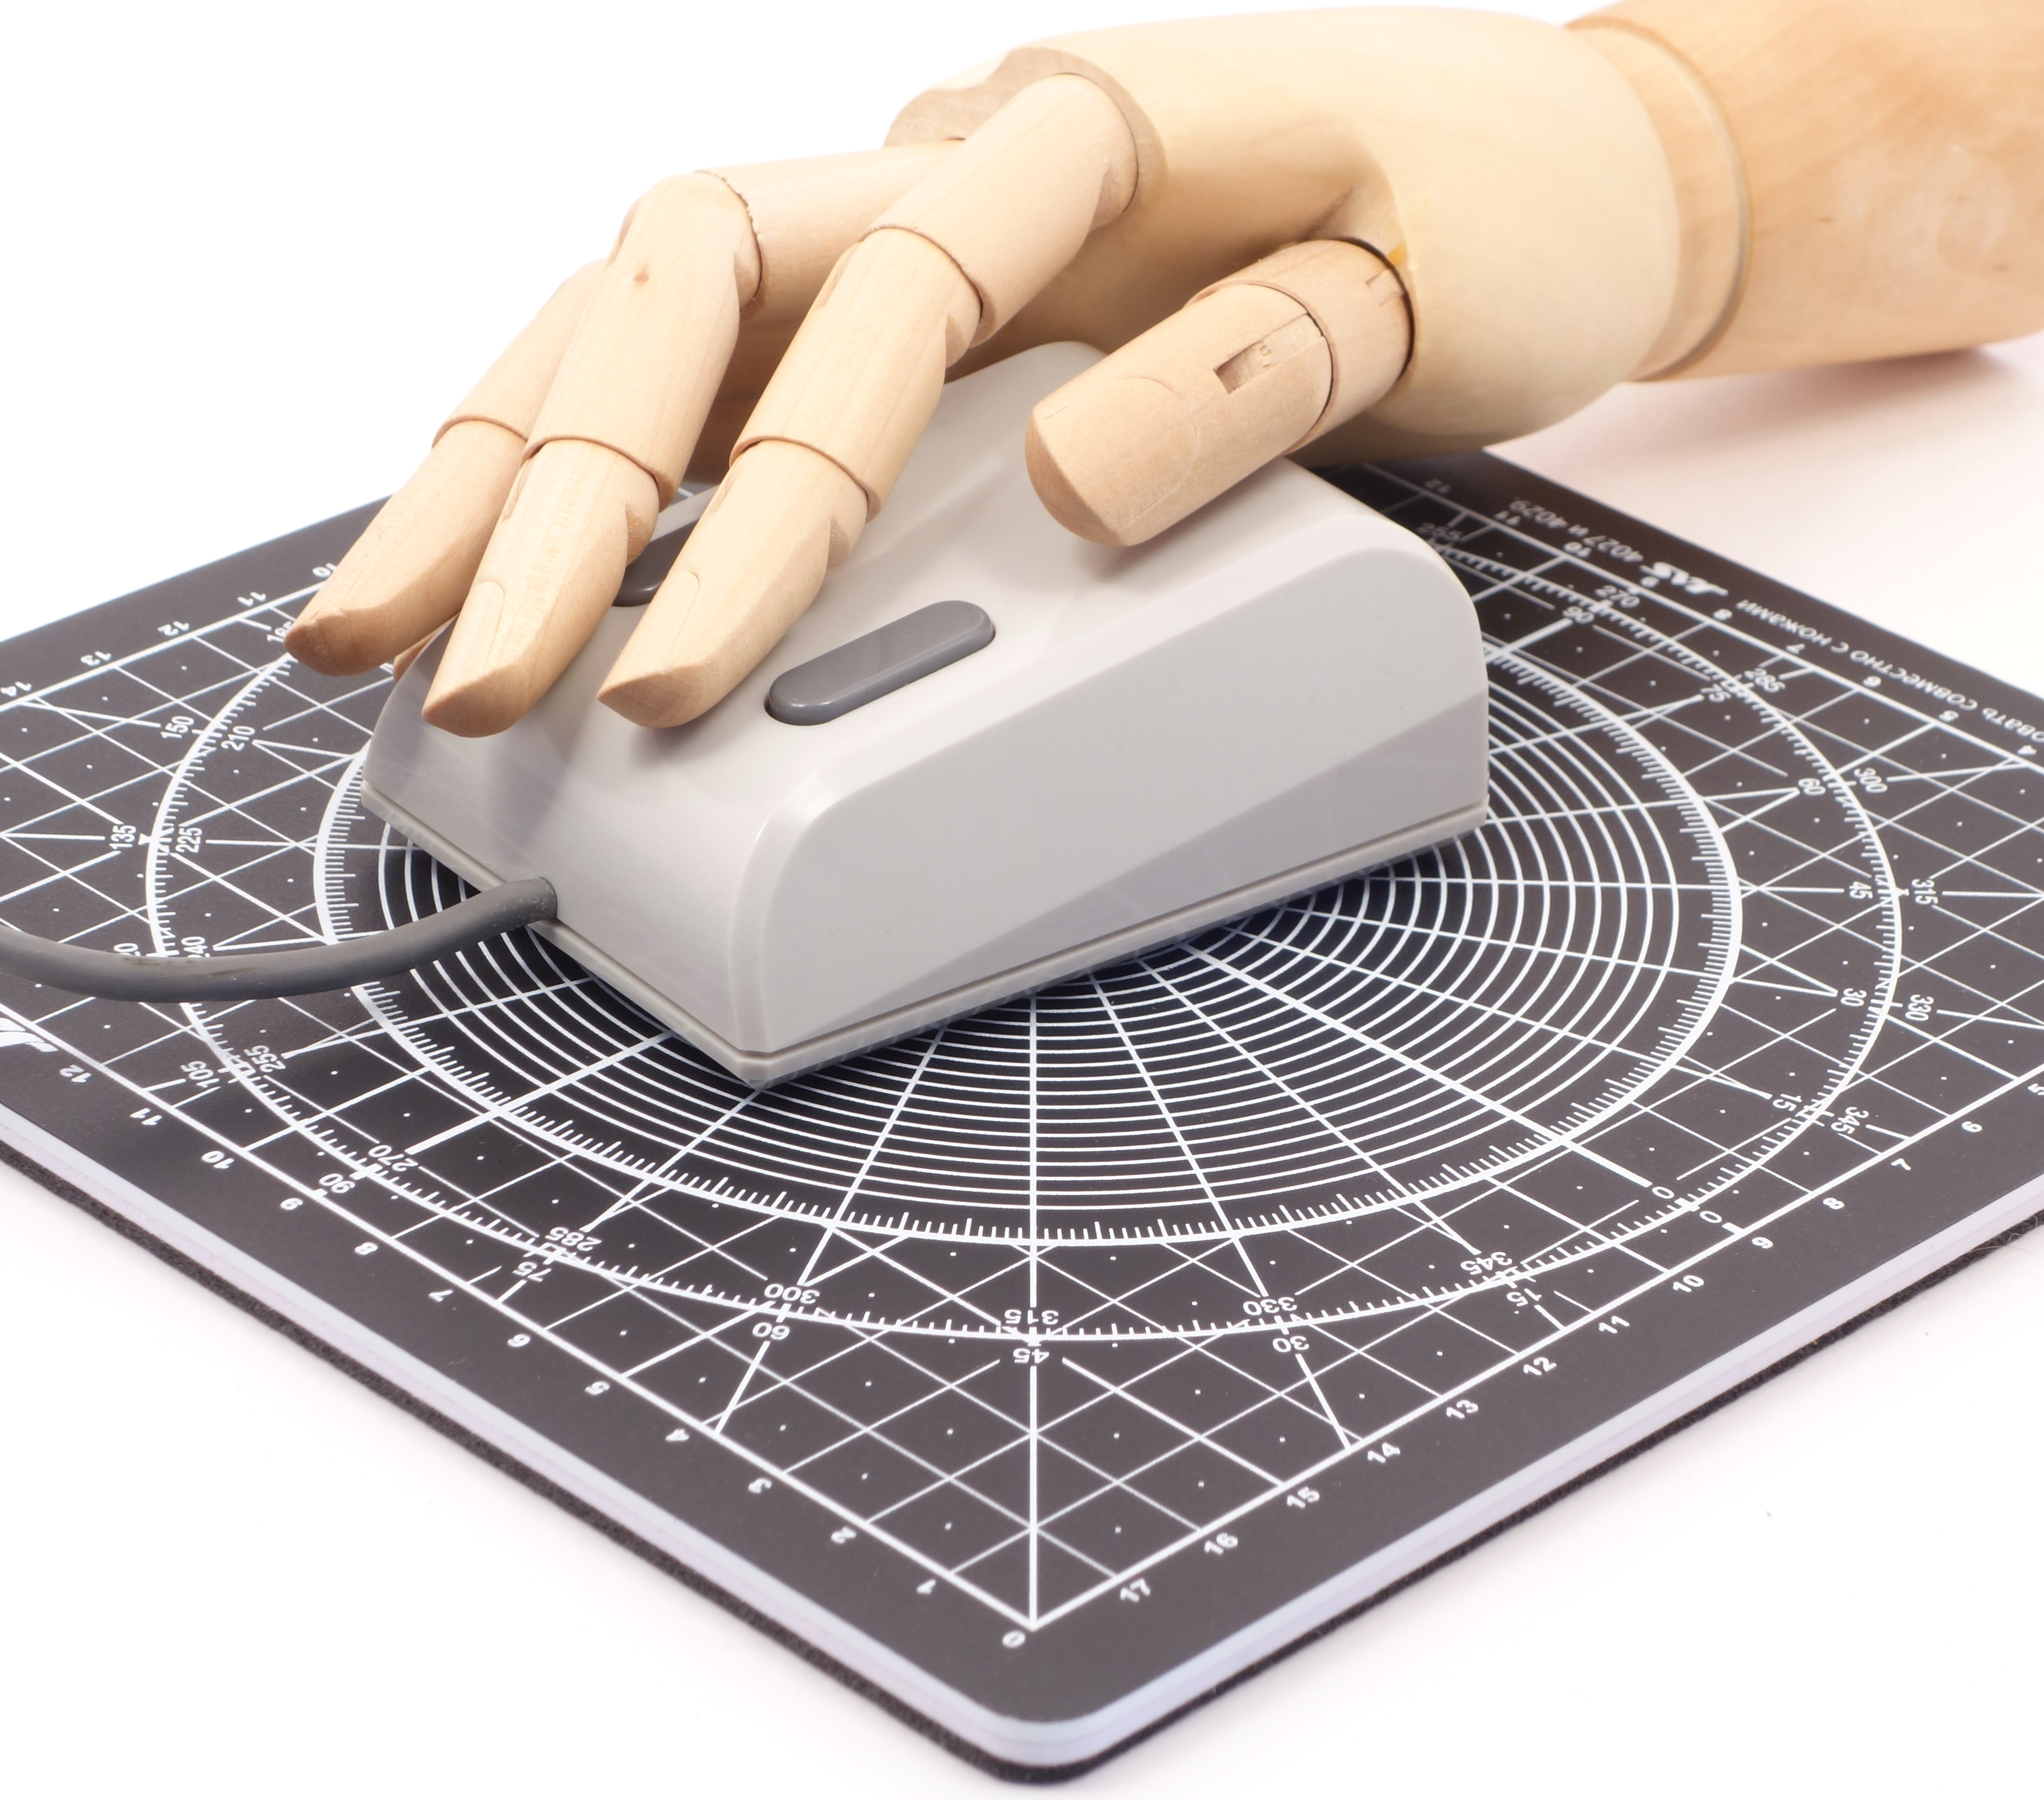
\includegraphics[scale=0.35]{1986_commodore_c300_mouse/cmruka_30.jpg}
    \caption{Commodore C300 Mouse with a human hand model}
    \label{fig:C300Hand}
\end{figure}

\begin{figure}[h]
    \centering
    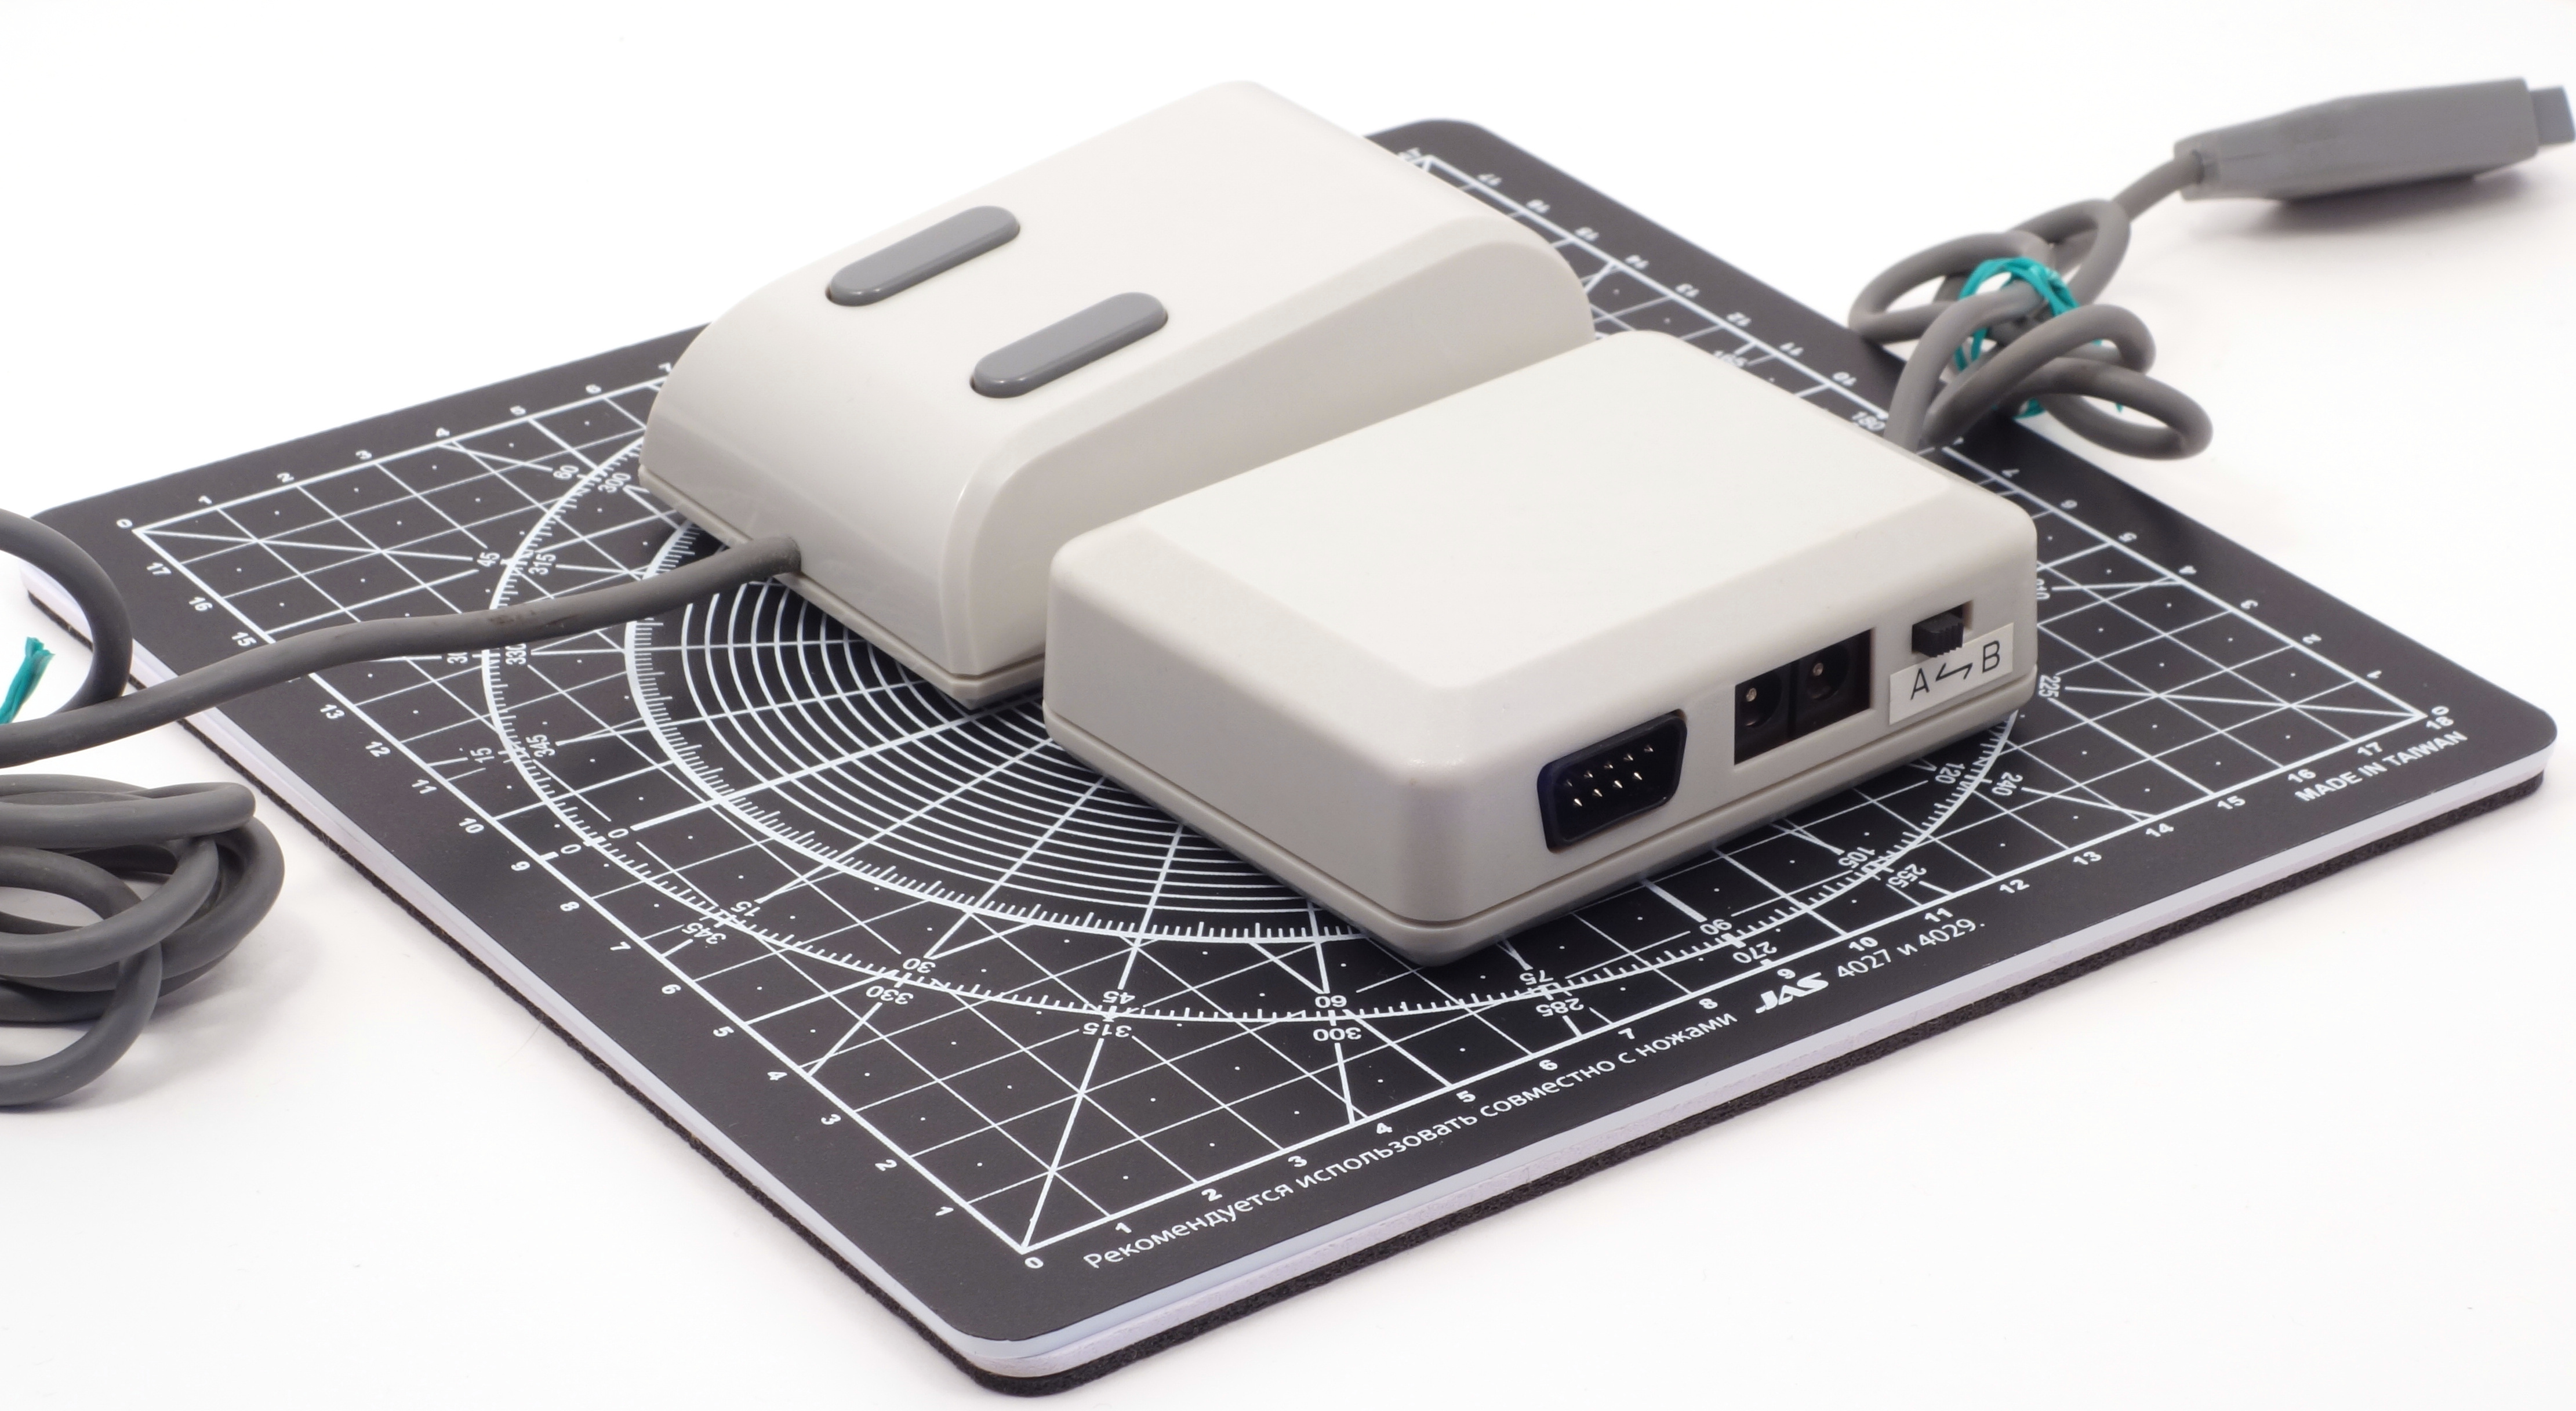
\includegraphics[scale=0.3]{1986_commodore_c300_mouse/cmblock_30.jpg}
    \caption{Commodore C300 mouse and adapter on a graduated pad with a grid step of 1~cm}
    \label{fig:C300Block}
\end{figure}

\begin{figure}[h]
    \centering
    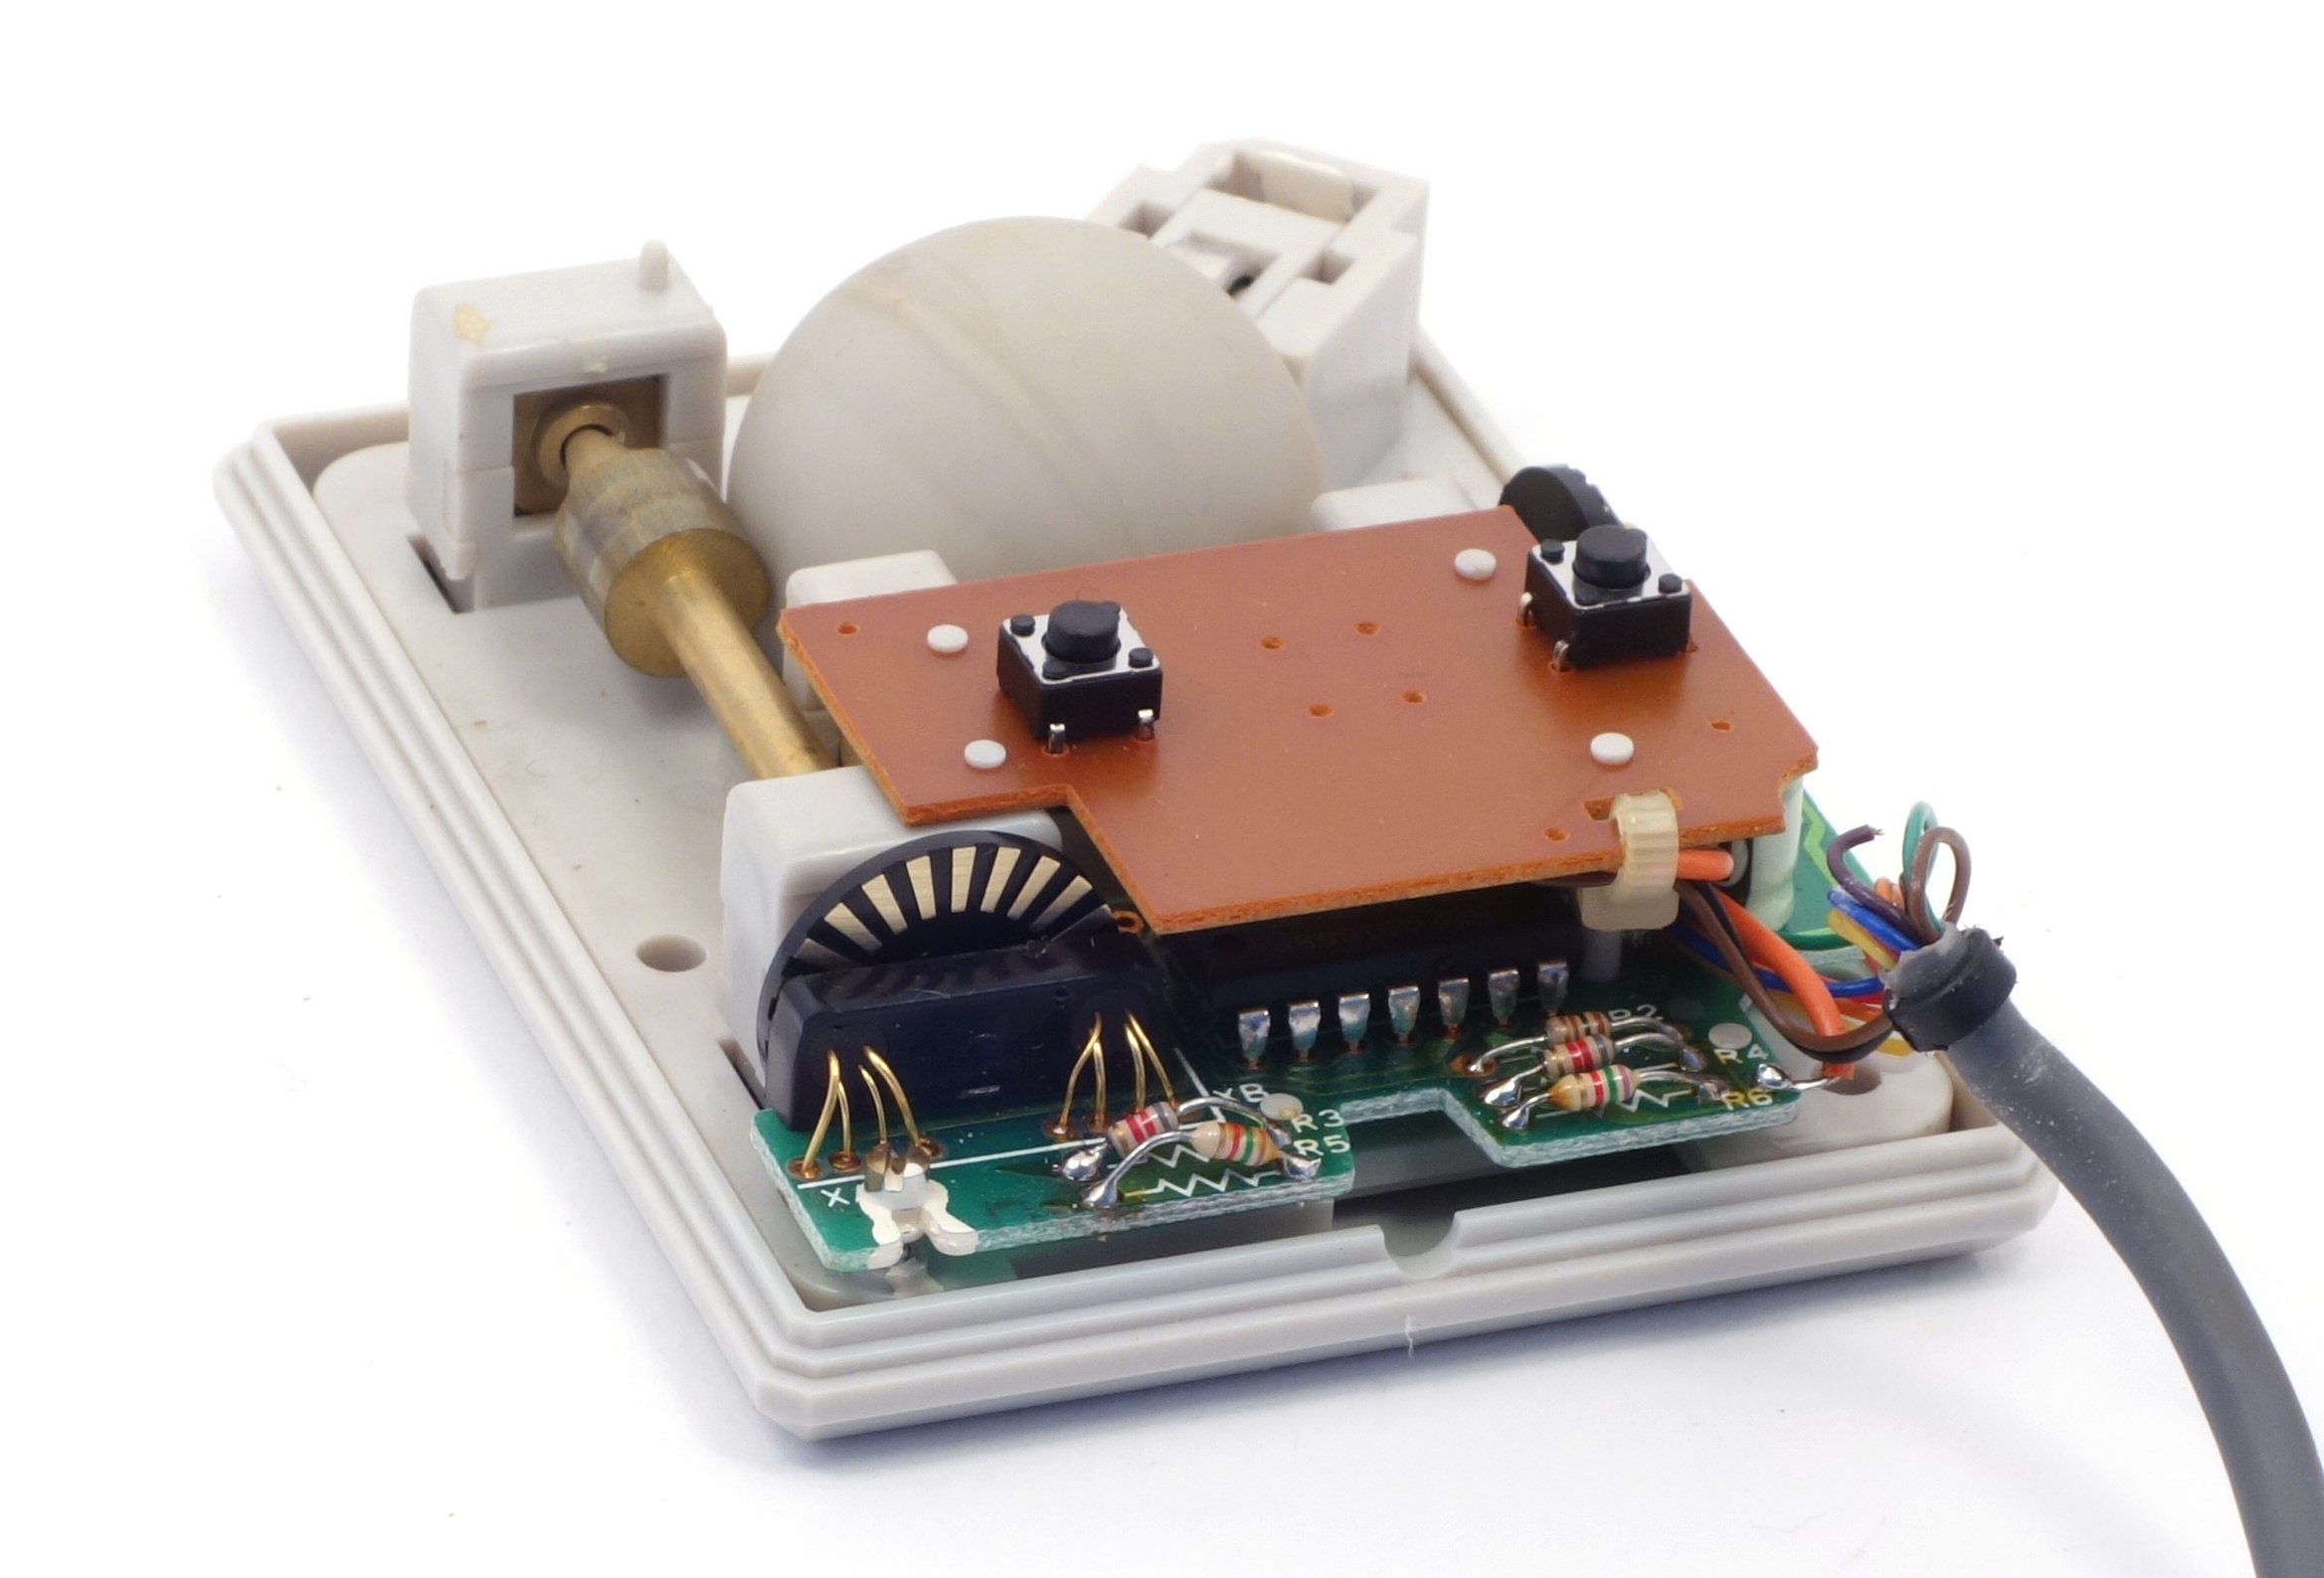
\includegraphics[scale=0.7]{1986_commodore_c300_mouse/cm4raz_30.jpg}
%    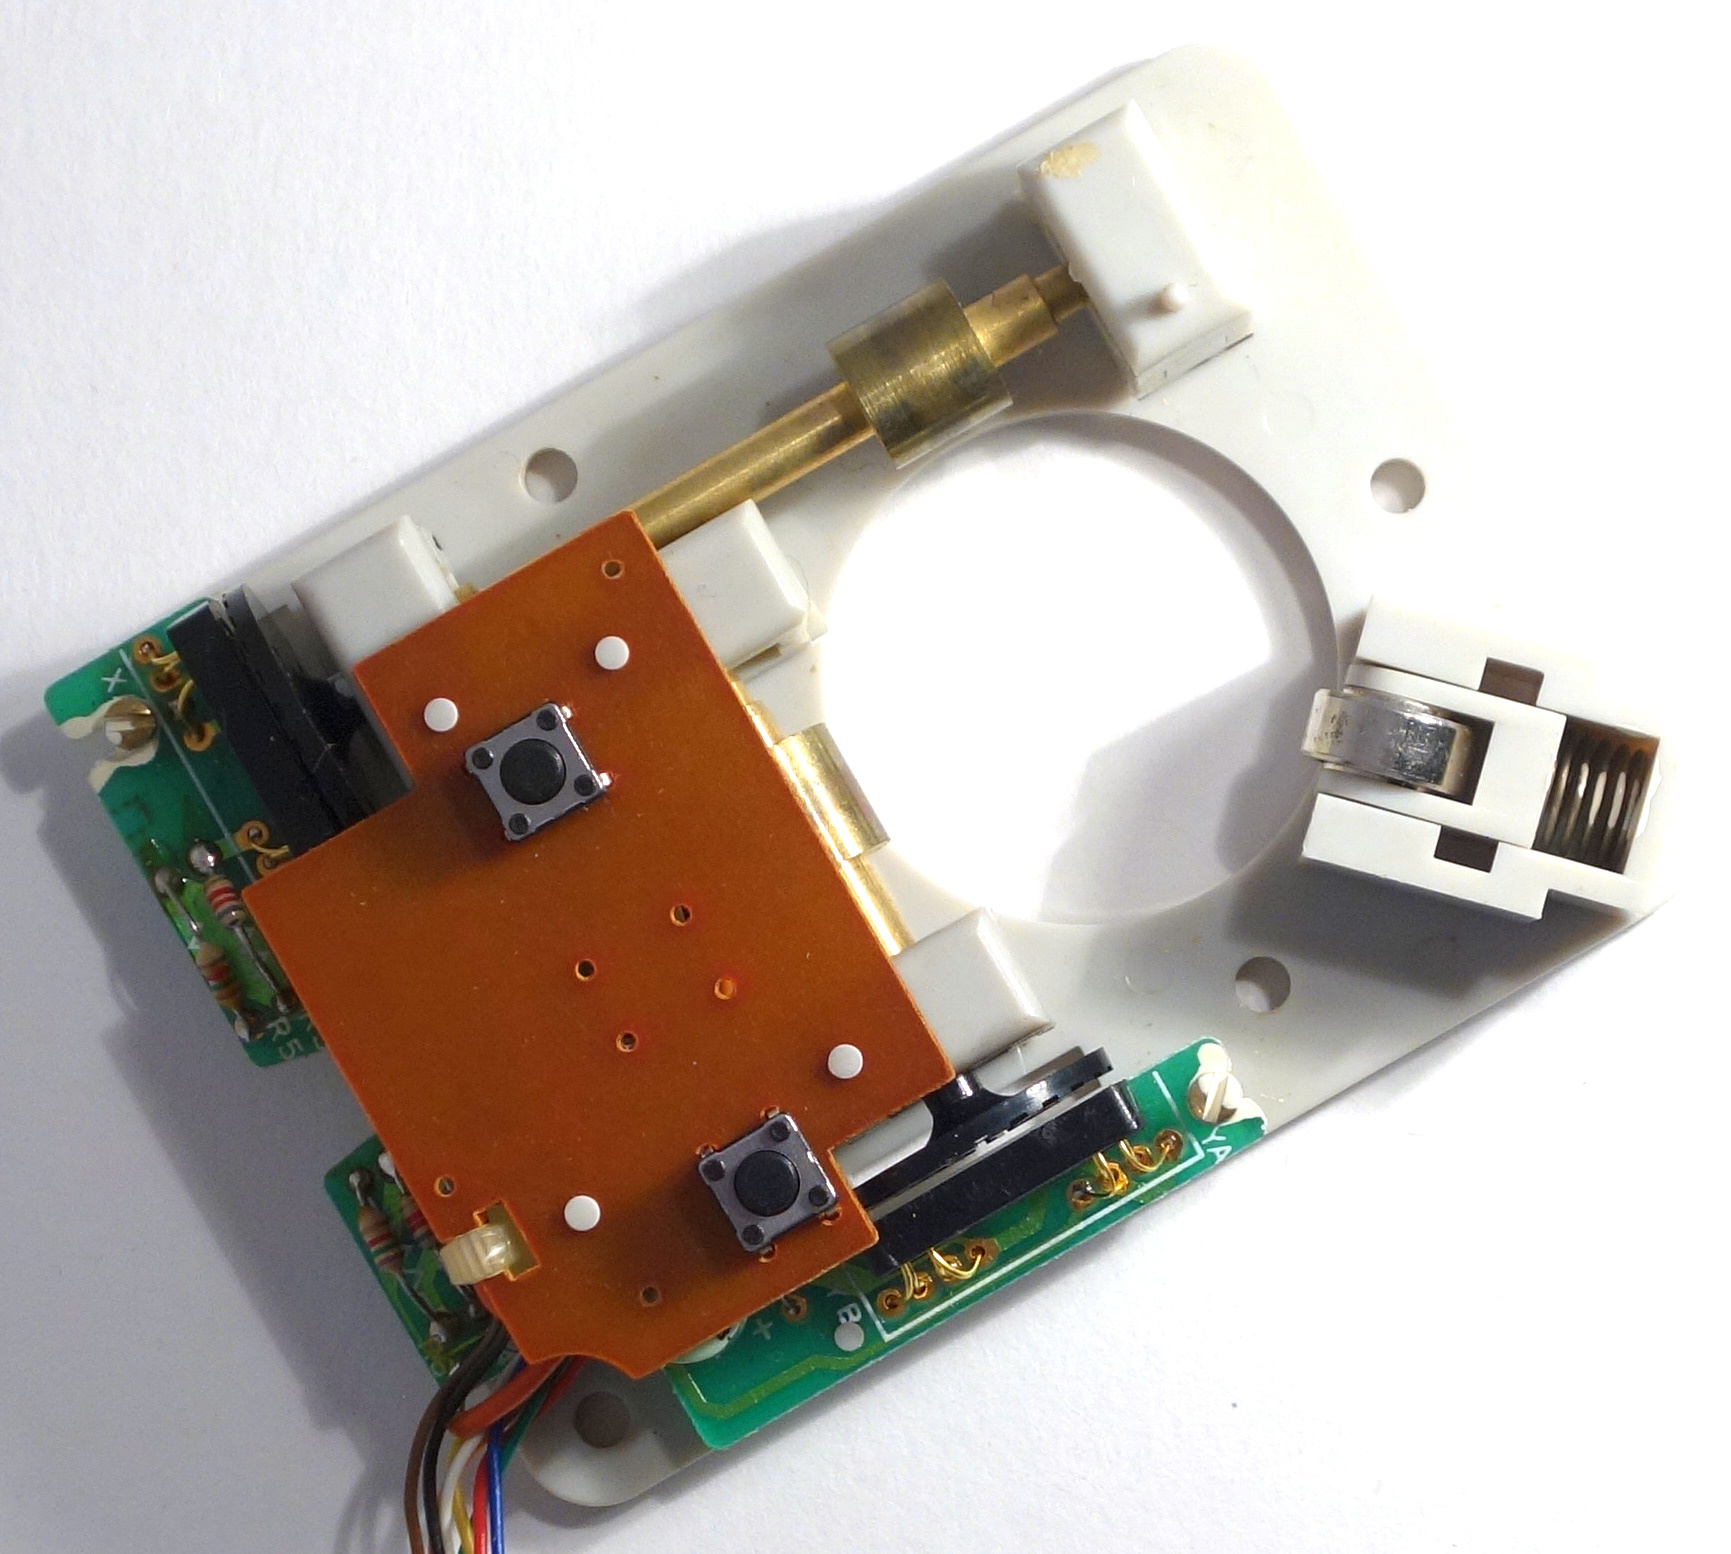
\includegraphics[scale=0.7]{1986_commodore_c300_mouse/cm41raz_30.jpg}
    \caption{Commodore C300 Mouse disassembled}
    \label{fig:C300Inside}
\end{figure}

Mouse internals are shown on figure \ref{fig:C300Inside}. The design is quite unusual: this is an original optomechanical pointing device with a non-standard optical interrupter. Instead of passing the disk between the light source and the optical detector, the LED and the photodiode are located on the same side of the disk, and the disk itself is Solid. Instead of slots, it used the radial metal strips reflecting light, while the black matte material of the disk itself scatters it, causing the absence of a signal on the photo receiver. In electrical terms, such a design does not differ from other opto-mechanical mice, but visually resembles a disk of contact encoder (in which the mechanical contact of the brushes with the surface of the disk occurs: there is an electrical contact at the time of the passing of a metal radial strip, and there is no contact when the brush is between the stripes).

Of course, such a solution is not cheap in comparison with a traditional scheme that uses a plastic disk with slots without metal.

\begin{thebibliography}{9}
\bibitem {c64wiki} Mouse -- C64-Wiki \url{https://www.c64-wiki.com/wiki/Mouse}
\bibitem {SinclairUser} Kempston mouse // Sinclair User, Iss. 56, November 1986. -- p. 29. \url{https://worldofspectrum.org/archive/magazines/sinclair-user/56/0/1986/11/0}
\end{thebibliography}
\end{document}
